\documentclass[12pt]{report}
\usepackage{StyleSheets/main}
\begin{document}

\chapter{Diagrams}\label{ap:diagrams}

\section{Robot Designs}
\label{sc:designs}

\begin{figure}[H]
    \centering
    \includegraphics[width=0.6\textwidth]{Images/Designs/Design1.pdf}
    \caption{Design 1 Conceptual Design}
    \label{fig:design1}
\end{figure}

\begin{figure}[H]
    \centering
    \includegraphics[width=1\textwidth]{Images/Designs/Design2.pdf}
    \caption{Design 2 Conceptual Design}
    \label{fig:design2}
\end{figure}

\begin{figure}[H]
    \centering
    \includegraphics[width=1\textwidth]{Images/Designs/Design3.pdf}
    \caption{Design 3 Conceptual Design}
    \label{fig:design3}
\end{figure}

\begin{figure}[H]
    \centering
    \includegraphics[width=1\textwidth]{Images/Designs/Design4.pdf}
    \caption{Design 4 Conceptual Design}
    \label{fig:design4}
\end{figure}

\section{Robot Images}

\begin{figure}[H]
    \centering
    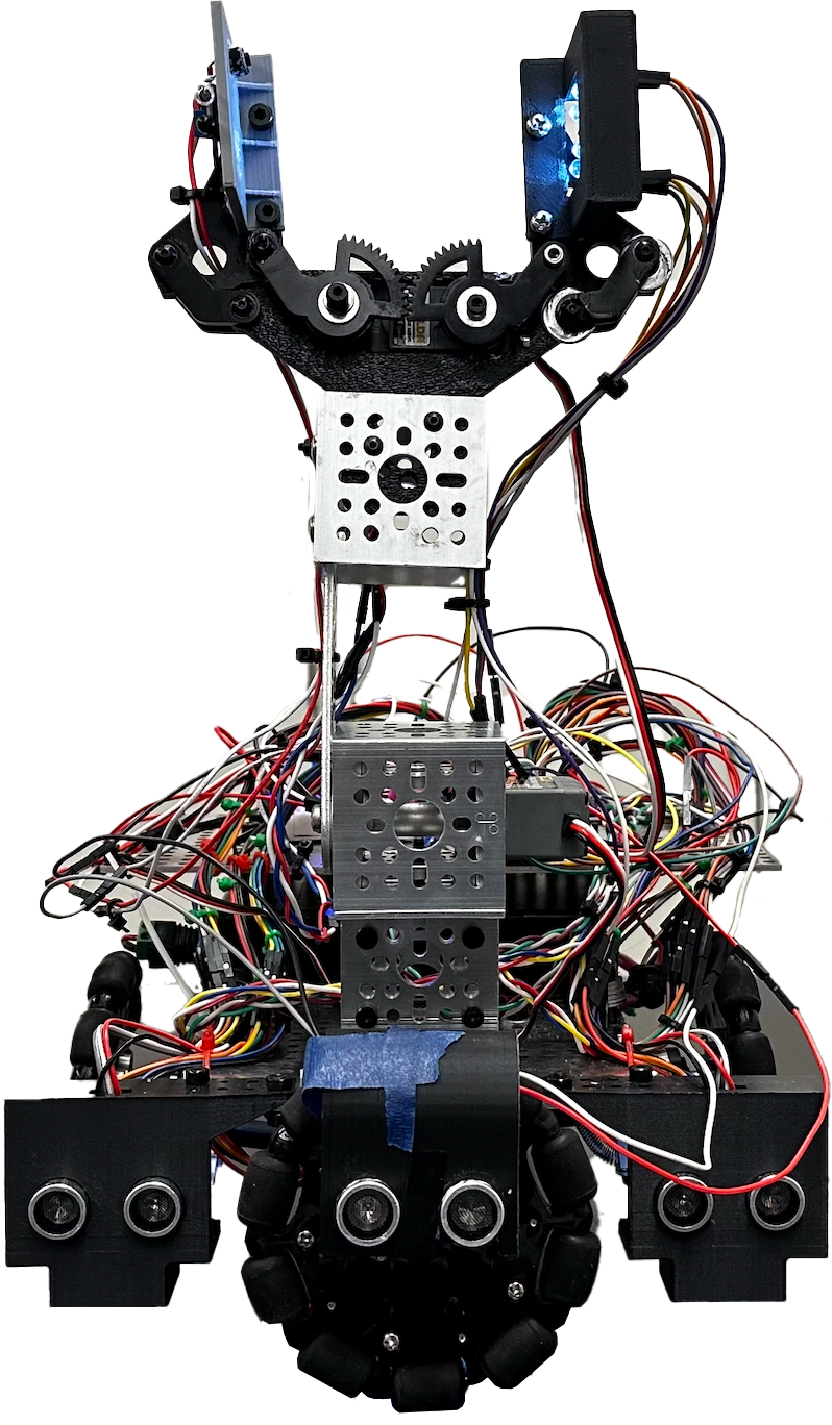
\includegraphics[width=0.7\textwidth]{Images/Robot/robot_front_view.pdf}
    \caption{Robot front view}
    \label{fig:front-view}
\end{figure}

\begin{figure}[H]
    \centering
    \includegraphics[width=0.68\textwidth]{Images/Robot/robot_underside.pdf}
    \caption{Robot underside}
    \label{fig:underside}
\end{figure}

\begin{figure}[H]
    \centering
    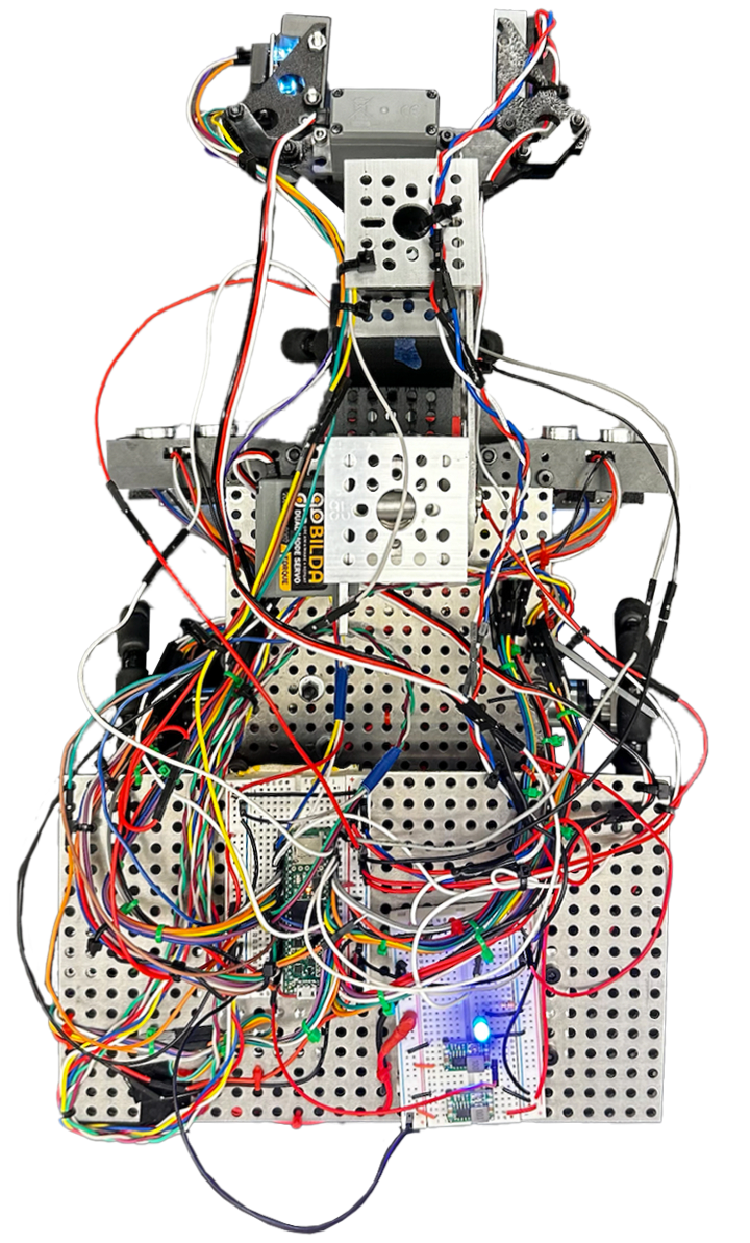
\includegraphics[width=0.8\textwidth]{Images/Robot/robot_top_view.pdf}
    \caption{Robot top view}
    \label{fig:topview}
\end{figure}

\section{3D Printed Parts}
\begin{figure}[H]
    \centering
    \includegraphics[width=1\textwidth]{Images/3D prints/USS_Front_new.PNG}
    \caption{Front Ultrasonic Sensor Mount}
    \label{fig:USS_front}
\end{figure}
\begin{figure}[H]
    \centering
    \includegraphics[width=1\textwidth]{Images/3D prints/CS-IR_M_new.PNG}
    \caption{Color Sensor - IR Sensor Mount}
    \label{fig:CS-IR mount}
\end{figure}


\begin{figure}[H]
    \centering
    \includegraphics[width=1\textwidth]{Images/3D prints/GRPR_CS_Long_new.PNG}
    \caption{Gripper Color Sensor Mount}
    \label{fig:GRPR_CS}
\end{figure}

\begin{figure}[H]
    \centering
    \includegraphics[width=1\textwidth]{Images/3D prints/GRPR_DualButton_new.PNG}
    \caption{Gripper Button Mount}
    \label{fig:GRPR_DualButton}
\end{figure}

\begin{figure}[H]
    \centering
    \includegraphics[width=1\textwidth]{Images/3D prints/USS-CS_Dual_new.PNG}
    \caption{Ultrasonic Sensor and Color Sensor Mounts}
    \label{fig:USS-CS_Dual}
\end{figure}

\begin{figure}[H]
    \centering
    \includegraphics[width=1\textwidth]{Images/Cost/slice1.pdf}
    \caption{Cost of first 3D-print.}
    \label{fig:printcost1}
\end{figure}

\begin{figure}[H]
    \centering
    \includegraphics[width=0.6\textwidth]{Images/Cost/slice2.pdf}
    \caption{Cost of second 3D-print.}
    \label{fig:printcost2}
\end{figure}

\begin{figure}[H]
    \centering
    \includegraphics[width=0.5\textwidth]{Images/Cost/slice3.pdf}
    \caption{Cost of third 3D-print.}
    \label{fig:printcost3}
\end{figure}

\begin{figure}[H]
    \centering
    \includegraphics[width=1\textwidth]{Images/Cost/ir_cost.pdf}
    \caption{Cost of the \gls{IR} sensor array.}
    \label{fig:enter-label}
\end{figure}

\section{Electrical Diagrams}
\subsection{Circuit Diagram}
\begin{figure}[H]
    \centering
    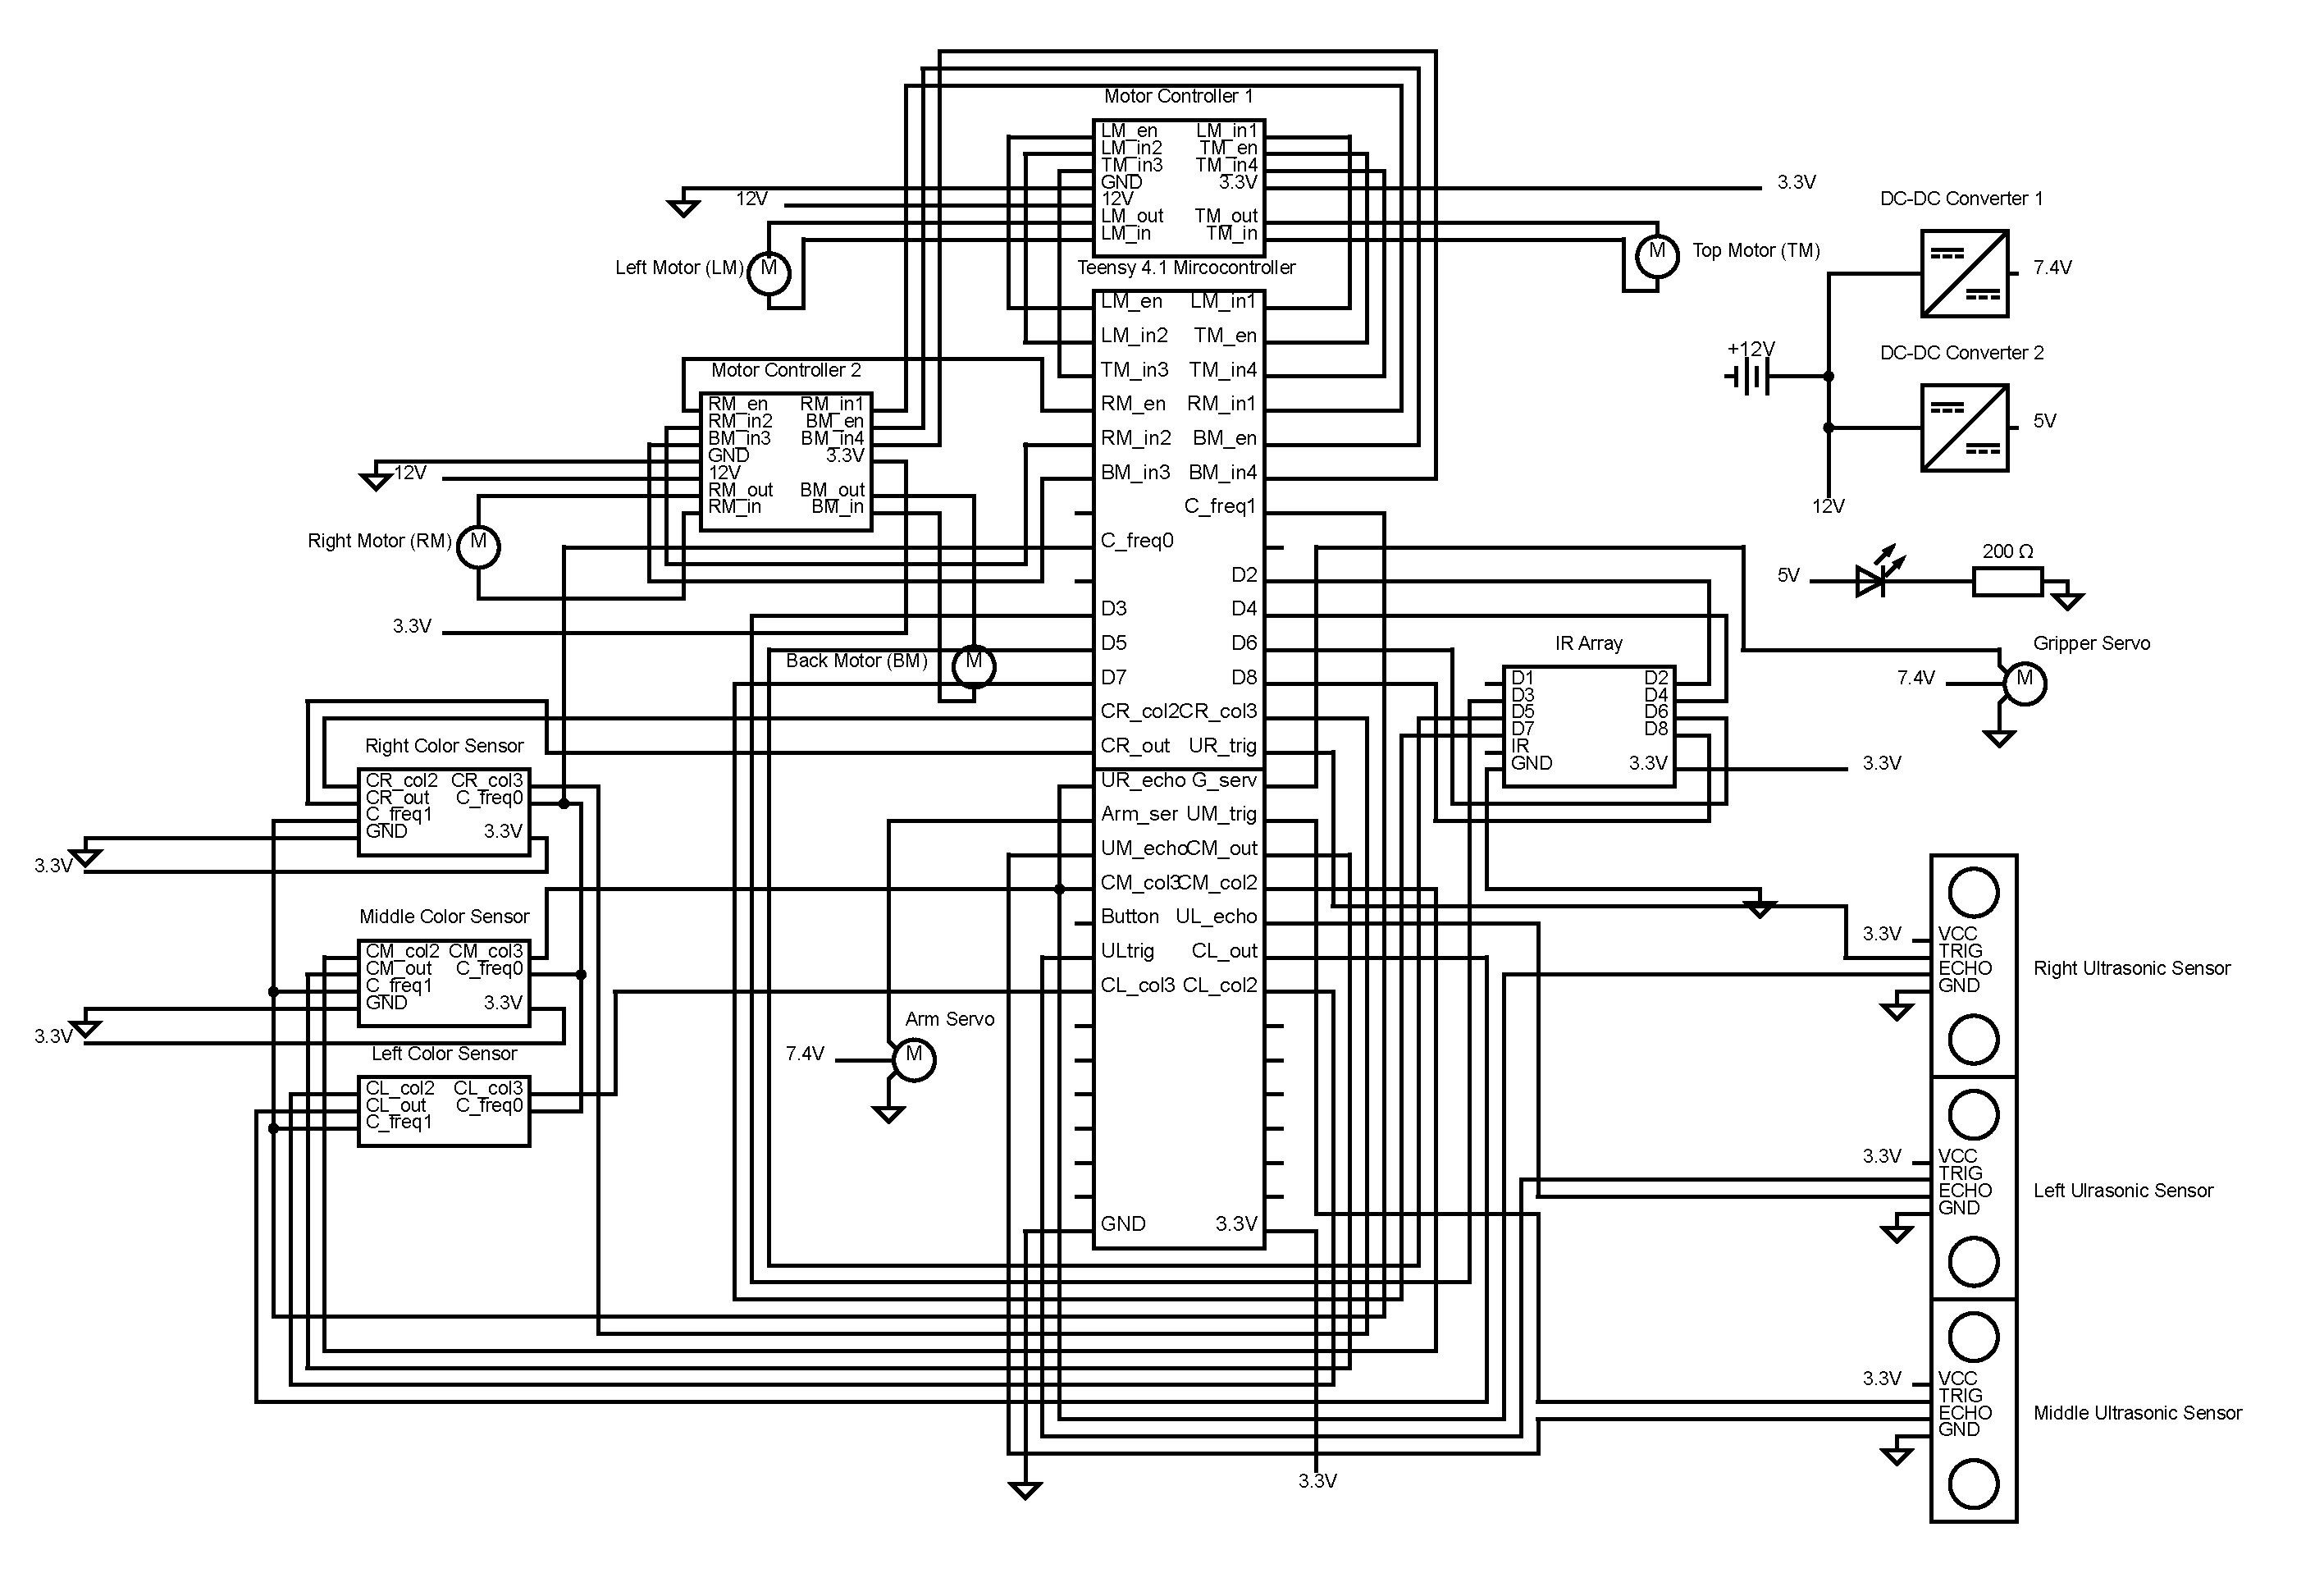
\includegraphics[width = 1.1\textwidth,angle=270, keepaspectratio]{Images/Diagrams/robot_pinout.pdf}
    \caption{Circuit Diagram}
    \label{fig:CircuitDiagram}
\end{figure}

\subsection{Pinout Map for Teensy 4.1}
\begin{figure}[H]
    \centering
    \includegraphics[width=1\textwidth]{Images/PinoutMap/Pinout map.PNG}
    \caption{Teensy 4.1 Microcontroller Pinout Map}
    \label{fig:Pinoutmap}
\end{figure}

\section{Pickup \& Place Flowchart}\label{sc:pickup-place-flowchart}

\begin{figure}[H]
    \centering
    \includegraphics[width=0.6\textwidth]{Images/flowchart/pid_line_following.pdf}
    \caption{PID Line Following Function}
    \label{fig:fc:pid_line_following}
\end{figure}

\begin{figure}[H]
    \centering
    \includegraphics[width=1\textwidth]{Images/flowchart/translational_line_centering.pdf}
    \caption{Translational Line Centering Function}
    \label{fig:fc:translational-line-centering}
\end{figure}

\begin{figure}[H]
    \centering
    \includegraphics[width=0.75\textwidth]{Images/flowchart/rotational_line_centering.pdf}
    \caption{Rotational Line Centering Function}
    \label{fig:fc:rotational-line-centering}
\end{figure}


\begin{figure}[H]
    \centering
    \includegraphics[width=0.5\textwidth]{Images/flowchart/begin.pdf}
    \caption{Beginning of Pickup \& Place}
    \label{fig:fc:begin}
\end{figure}

\begin{figure}[H]
    \centering
    \includegraphics[width=0.75\textwidth]{Images/flowchart/line_orientation.pdf}
    \caption{Line Orientation Sub Module}
    \label{fig:fc:line-orientation}
\end{figure}

\begin{figure}[H]
    \centering
    \includegraphics[width=1\textwidth]{Images/flowchart/middle_navigation.pdf}
    \caption{Middle Navigation Sub Module}
    \label{fig:fc:middle-navigation}
\end{figure}

\begin{figure}[H]
    \centering
    \includegraphics[width=1\textwidth]{Images/flowchart/fork_navigation.pdf}
    \caption{Fork Navigation Sub Module}
    \label{fig:fc:fork-navigation}
\end{figure}

\begin{figure}[H]
    \centering
    \includegraphics[width=0.8\textwidth]{Images/flowchart/find_platform.pdf}
    \caption{Find Platform Sub Module}
    \label{fig:fc:find-platform}
\end{figure}

\begin{figure}[H]
    \centering
    \includegraphics[width=1\textwidth]{Images/flowchart/navigate_back_to_fork.pdf}
    \caption{Navigate Back to Fork Sub Module}
    \label{fig:fc:navigate-back-to-fork}
\end{figure}

\begin{figure}[H]
    \centering
    \includegraphics[width=1\textwidth]{Images/flowchart/return_home.pdf}
    \caption{Return Home Sub Module}
    \label{fig:fc:return-home}
\end{figure}

\newpage\section{Pickup-and-Place Line Course}
\begin{figure}[H]
    \centering
    \includegraphics[width = 1.1\textwidth,angle = 270,keepaspectratio]{Images/Diagrams/pickup_place_course.pdf}
    \caption{Pickup-and-Place course.\protect\footnotemark}
    \label{fig:pickup-place-course}
\end{figure}
\footnotetext{Note that within the vertical, green lines are the boundaries of the randomized region of the course.}

\end{document}

    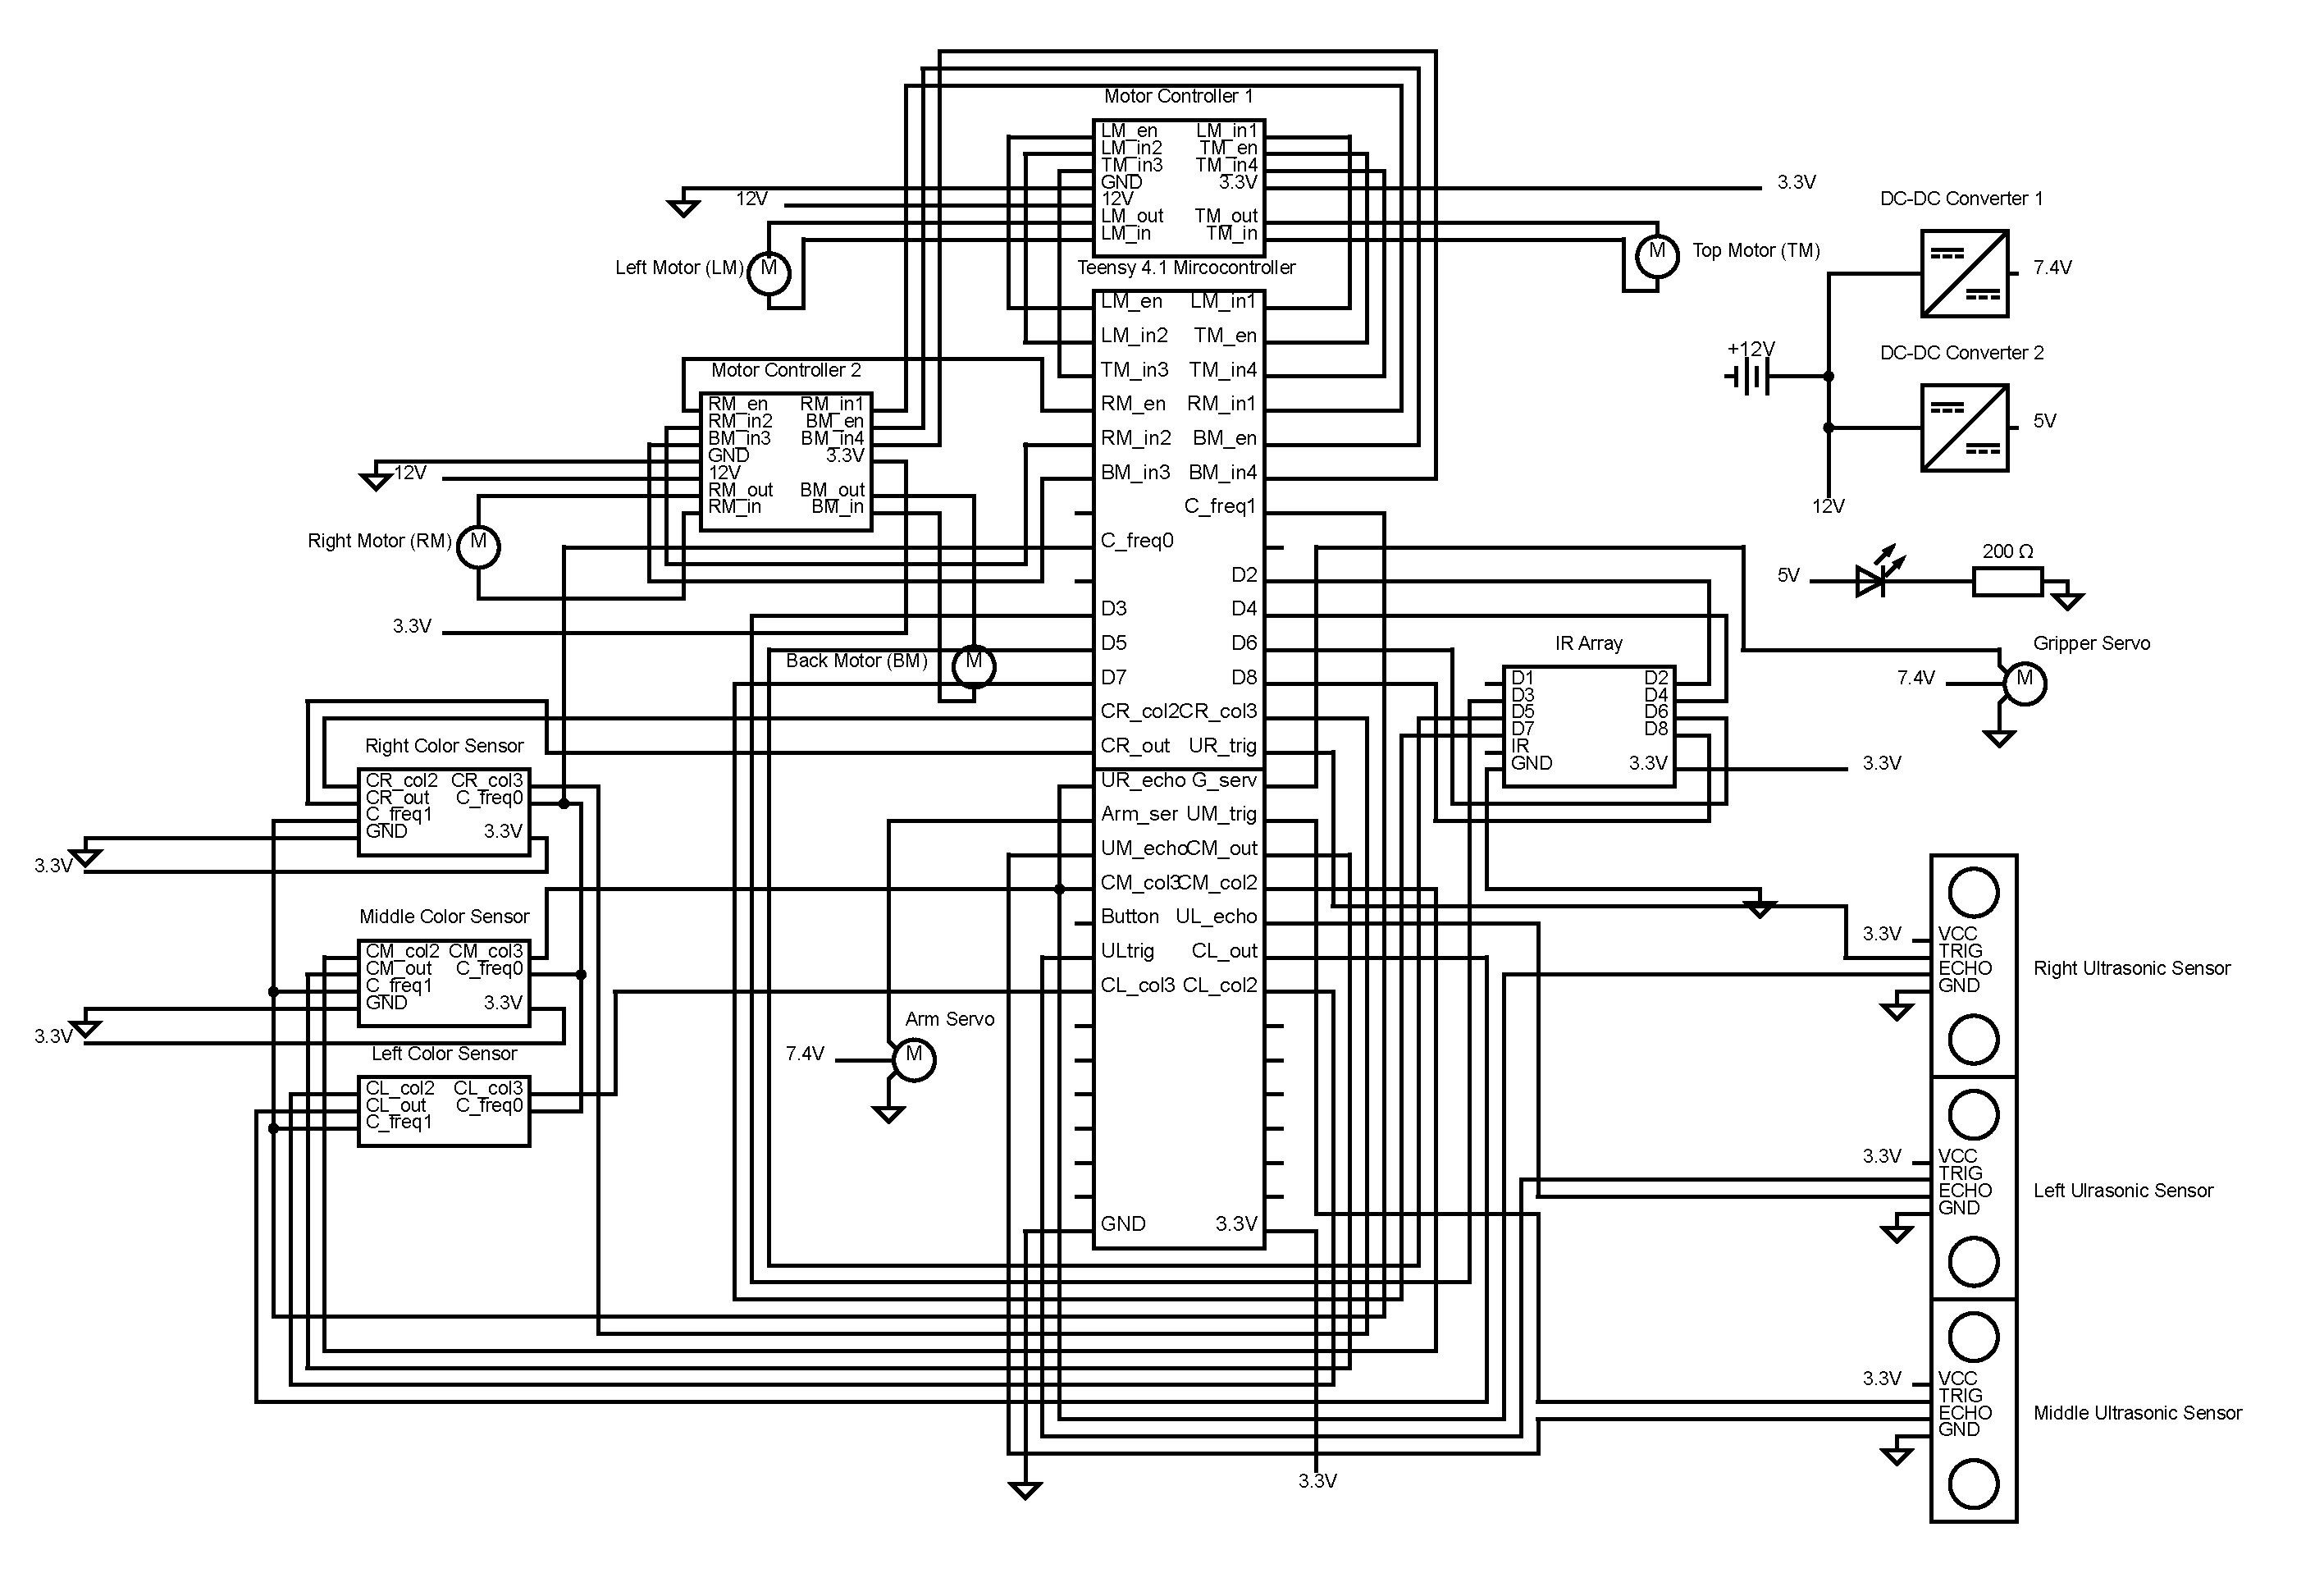
\includegraphics[width = 1.1\textwidth,angle=270, keepaspectratio]{Images/Diagrams/robot_pinout.pdf}
    \caption{Circuit Diagram}